\documentclass[
parskip=true,  % „german” paragraphs
fontsize=12pt, % or 11pt or 10pt
BCOR=12mm,     % binding correction
twoside=false  % no duplex printing -> no differnece between left and right pages
]{scrreprt}

% boiler plate. Sources musst be UTF-8, „new” german is the document language
% verwenden
\usepackage[utf8]{inputenc}
\usepackage[T1]{fontenc}
\usepackage[ngerman]{babel}

\usepackage{graphicx}  % \includegraphics
\usepackage{libertine} % Libertine font
\usepackage{blindtext} % \blindtext (only for layout test)
\usepackage{booktabs}  % cmidrule, toprule, midrule, bottomrule (nice tables)
\usepackage[printonlyused]{acronym}   % \ac
\usepackage[onehalfspacing]{setspace} % 1.5 line spacing
\usepackage{scrpage2}    % page header/foot
\pagestyle{scrheadings}  % use „live” header columns
\automark{chapter}       % use \chapter as header column
\usepackage{microtype}   % microtypograhpic enhancments
\usepackage{listings}    % Code Listings
% Default settings for code listings
\lstset{
    numbers=left,
    frame=shadowbox,
    showstringspaces=true,
    basicstyle=\footnotesize\ttfamily,
    captionpos=b
}

\usepackage{hyperref}

% hyperref/PDF settings
\hypersetup{
    colorlinks=true,
    linkcolor=black,
    citecolor=black,
    urlcolor=black,
    pdftitle={Masterarbeit von firstname lastname: Topic Topic Topic Topic},
    pdfauthor={firstname lastname <firstname.lastname@gmail.com>},
    pdfsubject={Topic Topic}
    pdfkeywords={Masterarbeit, fistname, lastname, Topic}
}

\begin{document}
% Here is everything in one document, obviously you want to split it up and use
% \include oder \input

% Title page
\begin{titlepage}
  \begin{center}
    \Large
    LMU München\\
    \large
    Fakultät für Irgendwas\\
    \vspace{15mm}
    \LARGE
    Masterarbeit\\
    \large
    von firstname lastname\\
    \vspace{15mm}
    \LARGE
    Topic Topic Topic Topic\\
    \vspace{15mm}
    \large
    Bearbeitungsbeginn\\
    \Large
    31. Februar 2055\\
    \vspace{5mm}
    \large
    Abgabetermin\\
    \Large
    31. Februar 2155\\
    \vspace{15mm}
    \large
    lfd.\,Nr.\\
    \Large
    42
  \end{center}
\end{titlepage}


% listings
\tableofcontents
\listoffigures
\listoftables

\chapter*{Abkürzungen}

\begin{acronym}
    \acro{API}{Application Programming Interface}
    \acro{BIOS}{Basic Input Output System}
    \acro{BSD}{Berkley Sofware Distributions}
\end{acronym}


\chapter{Einleitung}

\section{Definition}

% How to cite, see template.bib
Hier wird was definiert mit Quellenangabe\cite{wiki:muenchen}.

\blindtext

% emphasize text, typewriter text and reference to something
Und \emph{hier} kommt dann noch mehr \texttt{Text} mit einem Verweis auf
Abschnitt \ref{sec:motivation}.

\section{Motivation}
\label{sec:motivation} % see above for \ref

Hier steht die Motivation für alles\footnote{Oder auch nicht\cite{wiki:latex}}.
¿ÙtF–8 ŋêht æuch? Æ Typographie: »schweizer Anführungszeichen«, „deutsche
Anführungszeichen“, Apostrop’h, Bindestrich - Gedankenstrich –, amerikanischer
Gedankenstrich —.  Ausslassungspunkte … Ligaturen: ff, fi, ft. Siehe auch
Tabelle \ref{tab:tolletab} oder Abbildung \ref{abb:tollegrafik}.

\blindtext

\begin{itemize}
\item Eine
\item Liste
\item mit Punkten

\end{itemize}

\blindtext

\begin{table}[ht]
    \centering
    \begin{tabular}{rrrrr}
        \toprule
        Foo & Bar & Baz & Ram & Tam\\
        \midrule
        12 & 13 & 14 & 42 & 23\\
        \midrule
        1  & 2  &  3 & 12 &  7\\
        \bottomrule
    \end{tabular}
    \caption{Eine tolle Tabelle}
    \label{tab:tolletab}
\end{table}


\blindtext\blindtext

\begin{enumerate}
\item Eine
\item nummerierte
\item Liste
\end{enumerate}

\blindtext

\chapter{Noch ein großartiges Kapitel}

\blindtext\blindtext

% acronym as defined above
Erstes verwenden einer Abkürzung \ac{API} und jetzt zweites verwenden der
gleichen Abkürzung \ac{API}. Jetzt verwenden wir noch \ac{BIOS} und \ac{BSD}.

\blindtext

\minipage{\linewidth} % prevents page break inside code listing
\begin{lstlisting}[language=python,caption={Hello World},label=lst:hello]
# Hello World
def Hello():
    foo = 10;
    print "Hello World!"
\end{lstlisting}
\endminipage

Siehe Codebeispiel \ref{lst:hello}.

\blindtext

\begin{figure}[ht]
    \centering
    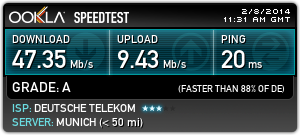
\includegraphics[width=0.8\textwidth]{img/bild.png}
    \caption{Eine tolle Grafik}
    \label{abb:tollegrafik}
\end{figure}

\blindtext

\begin{description}
\item[Begriff eins] Erläuterung für Begriff eins
\item[Begriff zwei] Erläuterung für Begriff zwei
\end{description}

\blindtext

\begin{equation}
    r_1^2 = x^2 + y^2
    \label{eq:kreis}
\end{equation}
\begin{equation}
    r_1 = \sqrt{x^2 + y^2}
    \label{eq:kreis2}
\end{equation}
\begin{equation}
    E = m \times c^2
    \label{eq:einstein}
\end{equation}

Ganz toll sind auch die Formeln \ref{eq:kreis} und \ref{eq:einstein}.

\blindtext

\bibliographystyle{geralpha}
\bibliography{template}

\end{document}
